Almost every tech company uses recommendation systems to provide its users a better experience. There are several types of methods to build a recommendation system. One of the most promising one is \ac{CORLP}. In this paper we have implemented \ac{CORLP} with MovieLens dataset.

\subsection{Recommendation Application}
First of all, I have built an application to implement recommendation system. This application is written in Python. I have used pandas, numpy and sklearn modules for implementing recommendation, gpcharts module for drawing charts.

\begin{figure}[h!]
   \centering
   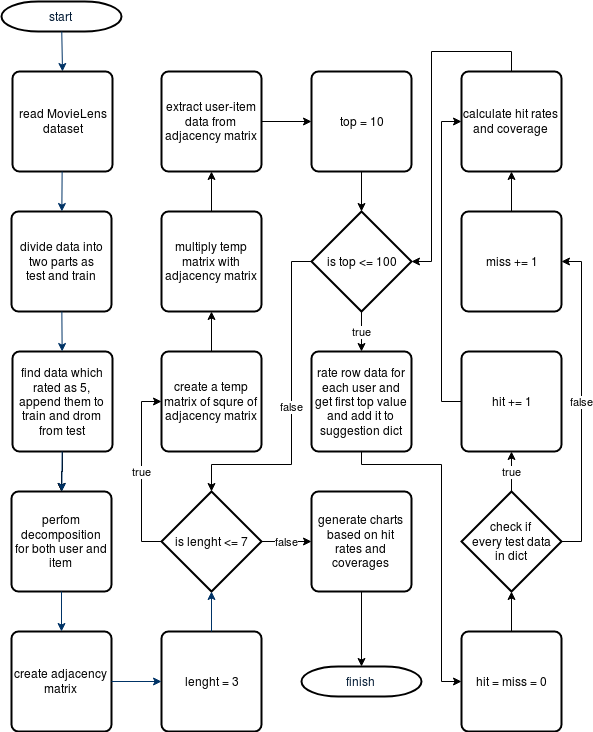
\includegraphics[width=1\linewidth]{images/flowchart.png}
   \caption{Flowchart}
   \label{fig:flowchart}
\end{figure}

As you can see in the figure ~\ref{fig:flowchart} application starts with reading dataset and dividing it into two parts as train and test data. It finds data which is rated as 5 from test data and moves the data from test to train. Perfoms decomposition for both users and items. Replaces NaN with 0, (1,2) with -j and (3,4,5) with j. Performs pearson correlation for both users and items. Creates adjacency matrix using user-user, user-item, item-user and item-item matrixes. Calculates square of adjacency matrix and assigns it to a temporary matrix. Creates a loop for 3, 5 and 7 lengths. Each time multiplies adjacency matrix with temporary matrix and assigns it to a result matrix. Extracts user-item matrix from result matrix. Performs test process if test data is in suggestion list. Performs counting operation based on the result. Calculates hit rates and coverage. Finally generates charts based on the results.

In this application, calculated length values are 3, 5 and 7. Suggestion sizes are 10 to 100 increments 10 each step.

MovieLens dataset contains 943 users, 1682 movies and 100k votes.

\subsection{Results}
As you can see in the figures ~\ref{fig:hits-rate-comparison} and ~\ref{fig:coverage-comparison} are results. For Top-10 and Lenght=3 hits rate is 8.61 and coverage is 10.12. For Top-100 and Lenght=3 hits rate is 44.92 and coverage is 52.17.

\begin{figure}[h!]
   \centering
   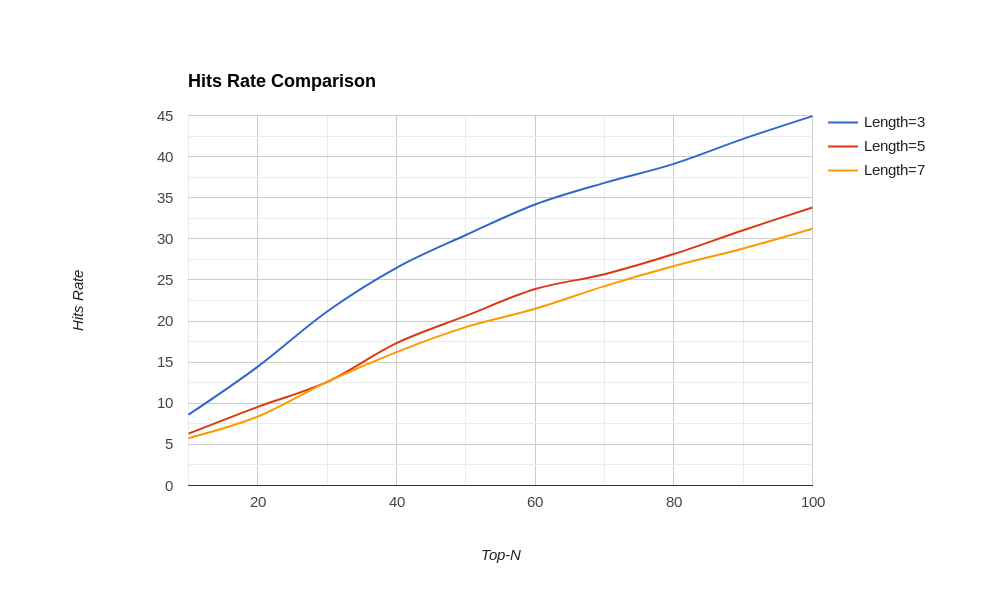
\includegraphics[width=1\linewidth]{images/hits-rate-comparison.png}
   \caption{Hits Rate Comparison}
   \label{fig:hits-rate-comparison}
\end{figure}

\begin{figure}[h!]
   \centering
   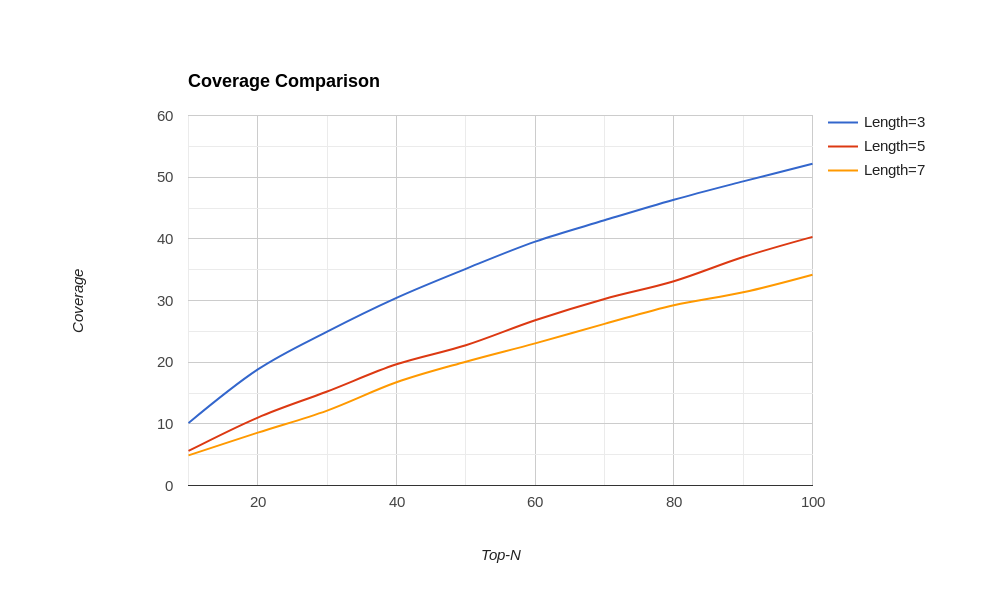
\includegraphics[width=1\linewidth]{images/coverage-comparison.png}
   \caption{Coverage Comparison}
   \label{fig:coverage-comparison}
\end{figure}